%%
%% Style file "borrowed" from Michel Goemans
%%
\documentclass[11pt]{article}

\usepackage{url,amsmath,amsthm,amsfonts,amssymb}
\usepackage{pgf}

\def\ceil#1{\lceil #1 \rceil}
\def\floor#1{\lfloor #1 \rfloor}
\def\ang#1{\langle #1 \rangle}

\newtheorem{definition}{Definition}
\newtheorem{remark}{Remark}
\newtheorem{theorem}{Theorem}
\newtheorem{lemma}[theorem]{Lemma}
\newtheorem{corollary}[theorem]{Corollary}
\newtheorem{proposition}[theorem]{Proposition}
\newtheorem{claim}[theorem]{Claim}
\newtheorem{observation}{Observation}

\newcommand{\R}{{\mathbb R}}
\newcommand{\Var}{\hbox{Var}}
\newcommand{\Z}{{\mathbb Z}}
\newcommand{\Q}{{\mathbb Q}}
\newcommand{\C}{{\mathbb C}}
\newcommand{\N}{{\mathbb N}}

\newlength{\toppush}
\setlength{\toppush}{2\headheight}
\addtolength{\toppush}{\headsep}

\newcommand{\htitle}[2]{\noindent\vspace*{-\toppush}\newline\parbox{6.5in}
 {\large Addis Ababa University, Amist Kilo \hfill #1\newline
\hspace*{\fill}{\bf Algorithms and Programming for High Schoolers} \hspace*{\fill} \newline
\mbox{}\hrulefill\mbox{}}\vspace*{1ex}\mbox{}\newline
\begin{center}{\Large\bf #2}\end{center}}

\newcommand{\handout}[3]{\thispagestyle{empty}
 \markboth{ #2}{ #2}
 \pagestyle{myheadings}\htitle{\protect\ref{#1}}{#2}{#3}}

\setlength{\oddsidemargin}{0pt}
\setlength{\evensidemargin}{0pt}
\setlength{\textwidth}{6.5in}
\setlength{\topmargin}{0in}
\setlength{\textheight}{8.5in}

\newcommand{\eps}{\varepsilon}
\newcommand{\sq}[1]{\langle#1\rangle}

\begin{document}

\htitle{August 5, 2016}{Lecture 15}

\paragraph{\Large Single-source shortest paths:}

We saw in Lab 10 that breadth-first search can be used to find the
shortest path between two vertices in a graph.  But what if the edges
in the graph have different lengths?  For example, in a graph
representing an airport network, edges have associated lengths
corresponding to the amount of time it takes to fly from one airport
to the next.  Then, we might not just be interested in getting from
one place to another in as few stops as possible, but we may instead
be interesting in minimizing total flight time.

A {\em weighted} graph is a triple $(V, E, w)$, where $w$ is a {\em
  weight} function.  Each edge $e\in E$ has a weight $w(e)$, which may
be positive, zero, or negative.  Now how can we find the shortest path
from one vertex to the others in such a graph?  This can be done using
recursion and memoization.  The non-recursive, iterative
implementation of this
approach is called the {\em Bellman-Ford} algorithm.

The basic idea is to create a recursive function
\texttt{shortestPathHelper}(x, y, t) which finds the shortest path
from $x$ to $y$ which takes at most $t$ steps.  One option is that it is the
same as the shortest path taking at most $t-1$ steps, and the other is
that we should travel to some vertex $z$ first in $t-1$ steps then
take the edge $(z,y)$ in the $t$th step.  We recurse on
both options and take the better of the two, and we use memoization to
make the function faster.
Note that if it's possible to get from $x$ to $y$ at all, then it is
possible to do so in $n-1$ steps, where the graph has $n$ vertices, so
the length of the shortest path from x to y is
\texttt{shortestPathHelper}(x, y, n-1).

\begin{figure}[!!h]
\begin{center}
\scalebox{0.5}{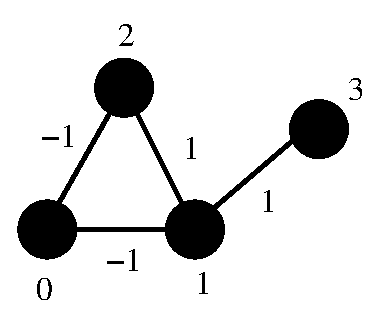
\includegraphics{weighted_graph}}
\end{center}
\caption{The numbers on edges are weights. This graph has a negative
  weight cycle $0\rightarrow 1\rightarrow 2\rightarrow 0$.}
\end{figure}

In some graphs though, such as those in Figure 1, there is no shortest
path from some vertex to another.  For example, to go from vertex $0$
to $3$, we could take the route $0\rightarrow 1\rightarrow 3$ for a
total length of $-1+1=0$.  However note that the cycle $0\rightarrow
1\rightarrow 2\rightarrow 0$ has a total length of $-1$.  Thus, by
repeatedly going on this cycle over and over again, we can make our
total length arbitrarily small before finally heading over to vertex
$3$.  Thus, in essence, the length of the shortest path from $0$ to
$3$ is $-\infty$.  We modify our \texttt{shortestPath} code to detect
such negative-weight cycles.  If any such cycle is found, starting
from our starting
vertex $x$, then we return $-1$.  Otherwise we return a list with all
the shortest path distances.

How can we detect a negative-weight cycle?  Let such a reachable cycle
be $v_0,v_2,\ldots,v_{k-1}$.  Let $d[u]$ be the shortest path distance
from $x$ to $u$ taking at most $n-1$ steps.  For the sake of
contradiction, assume that we cannot improve the distance to any of
the $v_i$ by looking at paths of length $n$.  That means that $d[v_i]
\le d[v_{i-1}] + w(v_{i-1}, v_i)$ for all $i$ (with the understanding
that $v_{-1}$ is just $v_{k-1}$).  Summing up all these inequalities
gives
$$ \sum_{i=1}^k d[v_i] \le \sum_{i=1}^k d[v_{i-1}] + \sum_{i=1}^k
w(v_{i-1}, v_i)$$
Since each $d[v_i]$ appears exactly once in the summations on
both sides, we can cancel to then get
$$ 0 \le \sum_{i=1}^k w(v_{i-1}, v_i) .$$
This is a contradiction, since we assumed that this cycle had negative
total weight.

Our implementation now follows.

\begin{verbatim}
# returns length of shortest path from x to y using at most t steps
def shortestPathHelper(B, x, y, t, mem, seen):
    if t == 0:
        if x == y:
            return 0
        return float(`infinity')
    elif seen[y][t]:
        return mem[y][t]

    seen[y][t] = True

    # first option: do it in t-1 steps
    ans = shortestPathHelper(B, x, y, t-1, mem, seen)

    # second option: go to a vertex z that has an edge to y first, in
    # at most t-1 steps, then take the edge (z, y)
    for p in B[y]:
        z = p[0]
        weight = p[1]
        val = shortestPathHelper(B, x, z, t-1, mem, seen)
        ans = min(ans, weight + val)
  
    mem[y][t] = ans
    return ans

# A is the adjacency list of the graph
# A[u][i][0] is the ith neighbor of vertex u, and A[u][i][1] is the
# weight of the edge (u, A[u][i][0])
#
# returns a list L so that L[j] is the length of the shortest path
# from x to j, assuming no negative-weight cycle is reachable from
# i. returns -1 if a negative-weight cycle is reachable from i.
def shortestPath(A, x):
    mem = []
    # mem[i][j] is float(`infinity') if we can't get from x to i in at
    # most j steps. Otherwise, it's the length of the shortest path
    # from x to i taking at most j steps.
    for i in xrange(len(A)):
        mem += [[float(`infinity')]*(len(A)+1)]

    seen = []
    # seen[i][j] is True if we've already filled in mem[i][j] and is
    # False otherwise
    for i in xrange(len(A)):
        seen += [[False]*(len(A)+1)]

    # B is an inverse adjacency list.  B[i] is a list of all vertices
    # j such that (j, i) is an edge, plus the weight of the edge
    B = []
    for i in xrange(len(A)):
        B += [[]]
    for i in xrange(len(A)):
        for p in A[i]:
            # p is the pair [j, weight(i, j)]
            B[p[0]] += [[i, p[1]]]

    # check if a negative weight cycle is reachable from x
    for z in xrange(len(A)):
        val1 = shortestPathHelper(B, x, z, len(A) - 1, mem, seen)
        val2 = shortestPathHelper(B, x, z, len(A), mem, seen)
        if val2 < val1:
            return -1

    L = []
    for y in xrange(len(A)): 
        L += [shortestPathHelper(B, x, y, len(A) - 1, mem, seen)]
    return L
\end{verbatim}

Na\"{i}vely one could say that the running time of the algorithm is
$O(n^3)$: in the memoized helper function there are $n$ choices for
$y$, $n$ choices for $t$, and the loop over B[y] might run for $n-1$
steps.  For some graphs this could happen, but in fact the algorithm's
running time is $\Theta(n(m+n))$, where the graph has $m$ edges.
$nm$ is
always at most $n^3$ since $m$ is at most $n^2$, but it can be a lot
faster if the graph doesn't have too many edges.  The reason the
running time is $\Theta(n(m+n))$ is the following.  
Look at the \texttt{for} loop ``\texttt{for p in B[y]}'' in
\texttt{shortestPathHelper}.  The total number of $(p,y)$ values this
loop executes with is exactly $m$: each $(p,y)$ pair corresponds to an
edge in the graph.  Then, there are $n$ possible values of $t$, giving
$nm$.  

The $n^2$ term comes from there being $n$ possible values of
both $y$ and $t$, though this term can be removed with a better
implementation, which we give below. The below implementation is an
iterative implementation of the approach above, but written 
iteratively instead of recursively.  It is known as the Bellman-Ford
algorithm.  The code is also quite a bit shorter than the recursive
implementation given above.

\newpage

\begin{verbatim}
def bellmanFord(A, x):
    # E is a list of edges with weights
    E = []
    for i in xrange(len(A)):
        for p in A[i]:
            E += [[i] + p]
    # dist[i] is the length of the shortest path to i
    dist = [float(`infinity')]*len(A)
    dist[x] = 0
    for i in xrange(len(A) - 1):
        for e in E:
            u = e[0]
            v = e[1]
            weight = e[2]
            dist[v] = min(dist[v], dist[u] + weight)

    # look for negative weight cycles
    for e in E:
        u = e[0]
        v = e[1]
        weight = e[2]
        if dist[u] + weight < dist[v]:
            return -1

    L = []
    for i in xrange(len(A)):
        L += [dist[i]]
    return L
\end{verbatim}

\paragraph{\Large All pairs shortest paths:}
What about finding all shortest path lengths between all pairs of
vertices?  Here we use memoization yet again.  
Let's assume the graph has no negative weight cycles.
An iterative, non-recursive version of
the below approach is known as the {\em Floyd-Warshall} algorithm. 

The
approach is to let \texttt{shortestPathHelper}(u, v, k) be the length of the
shortest path where the intermediate vertices come from the set
$\{0,1,\ldots,k-1\}$.  For such a shortest path we have two choices:
either don't use vertex $k-1$ at all, so that the answer is
\texttt{shortestPathHelper}(u, v, k-1), or use it so that the answer is
\texttt{shortestPathHelper}(u, k-1, k-1) + \texttt{shortestPathHelper}(k-1, v,
k-1).  When $k=0$ we cannot use intermediate vertices, which means the
answer is just the weight of the edge from $u$ to $v$.

\begin{verbatim}
def shortestPathHelper(u, v, k, w, mem, seen):
    if k == 0:
        return w[u][v]
    elif seen[u][v][k]:
        return mem[u][v][k]

    seen[u][v][k] = True
 
    option1 = shortestPathHelper(u, v, k-1, w, mem, seen)
    val1 = shortestPathHelper(u, k-1, k-1, w, mem, seen)
    val2 = shortestPathHelper(k-1, v, k-1, w, mem, seen)
    mem[u][v][k] = min(option1, val1 + val2)
    return mem[u][v][k]

# w is a matrix of edge weights, i.e. w[i][j] is the weight of the
# edge (i,j). If that edge doesn't exist, we assume w[i][j] is then
# float(`infinity')
def shortestPath(w):
    ans = []
    for i in xrange(len(w)):
        ans += [[-1]*len(w)]

    mem = []
    for i in xrange(len(w)):
        l = []
        for j in xrange(len(w)):
            l += [[-1]*(len(w)+1)]
        mem += [l]

    # seen[i][j][k] is True if we've already filled in mem[i][j][k],
    # and it is False otherwise
    seen = []
    for i in xrange(len(w)):
        l = []
        for j in xrange(len(w)):
            l += [[False]*(len(w)+1)]
        seen += [l]
    
    for i in xrange(len(w)):
        for j in xrange(len(w)):
            ans[i][j] = shortestPathHelper(i, j, len(w), w, mem, seen)
    return ans
\end{verbatim}

In fact, a non-recursive implementation of this approach is much
slicker and amounts to just three \texttt{for} loops.  This is known
as the Floyd-Warshall algorithm.  It also uses less memory than the
implementation above ($\Theta(n^2)$ instead of $\Theta(n^3)$).

\newpage

\begin{verbatim}
def floydWarshall(w):
    # now dist is a copy of the weight function
    dist = w[:]

    for k in xrange(len(w)):
        for u in xrange(len(w)):
            for v in xrange(len(w)):
                dist[u][v] = min(dist[u][v], dist[u][k] + dist[k][v])
    return dist  
\end{verbatim}

Both the iterative and recursive implementations of Floyd-Warshall
above take $\Theta(n^3)$ time, though the iterative implementation
requires less memory.
\end{document}
